\section{Theorie}
\label{sec:Theorie}
\subsection{Allgemein}
Wirken Kräfte auf einen Körper, so kann die Form und das Volumen des Körpers verändert werden.
Die Kräfte beziehen sich meist auf die Flächeneinheit und werden als Spannung $\sigma$ bezeichnet.
Die senkrecht zur Oberfläche wirkende Spannung wird als Normalspannung bezeichnet.
Tangential- oder Schubspannung heißt hingegen die parallel zur Oberfläche verlaufende Komponente.
Liegt bei der relativen Längenänderung $\frac{\Delta L}{L}$ ein linearer Zusammenhang vor, so beschreibt das Hook'sche Gesetz
\begin{equation}
    \sigma = E \cdot \frac{\Delta L}{L}
\end{equation}
die Deformation.
Dabei beschreibt $E$ der Elastizitätsmodul, $L$ die Länge und $\Delta L$ die Längenänderung des Körpers (siehe Abb. \ref{fig:spannung}).
Der Elastizitätsmodul ist eine materialabhängige Konstante des Werkstoffes.
Die Längenänderung $\Delta L$ kann nur mit genauen Messaperaturen direkt bestimmt werden.\\
Eine weitere Möglichkeit zur Bestimmung des Elastizitätsmodul ist die Biegung.
Hier genügt eine relativ kleine Kraft am Ende des Stabes um eine messbare Längenänderung zu bewirken.
\begin{figure}
    \centering
    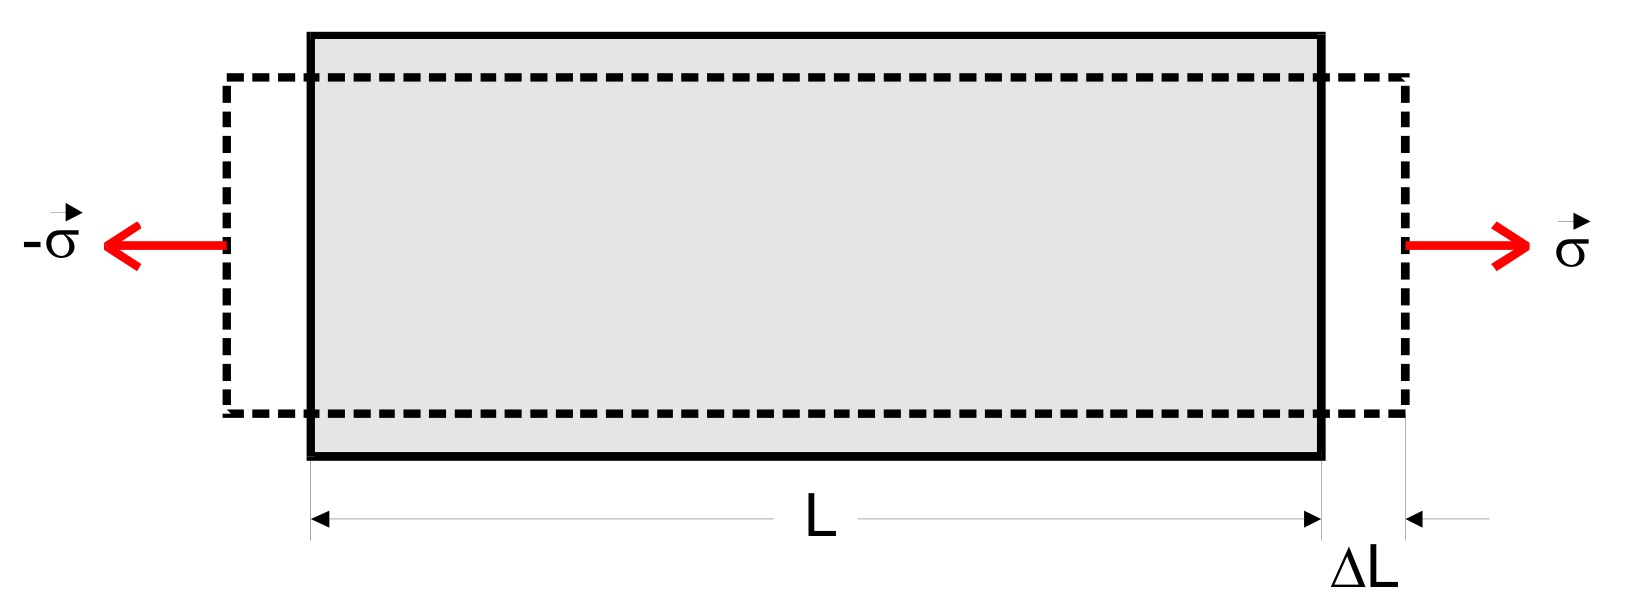
\includegraphics[width=0.75\textwidth]{content/data/spannung.jpg}
    \caption{Dehnung eines Stabes bei wirkender Normalspannung.\cite{anleitung}}
    \label{fig:spannung}
\end{figure}
\subsection{Biegung - Einseitige Einspannung}
Ein homogener Stab wird auf einer Seite eingespannt und am anderen Ende wirkt eine Kraft $F$.
Es wird die Durchbiegung $D(x)$ gemessen.
Sie beschreibt die Verschiebung von einem Oberflächenpunkt bei einer Biegung (siehe Abb. \ref{fig:stab_einseitig}).
Mithilfe von $x$ und $D(x)$ kann die Materialkonstante bestimmt werden.
\begin{figure}
    \centering
    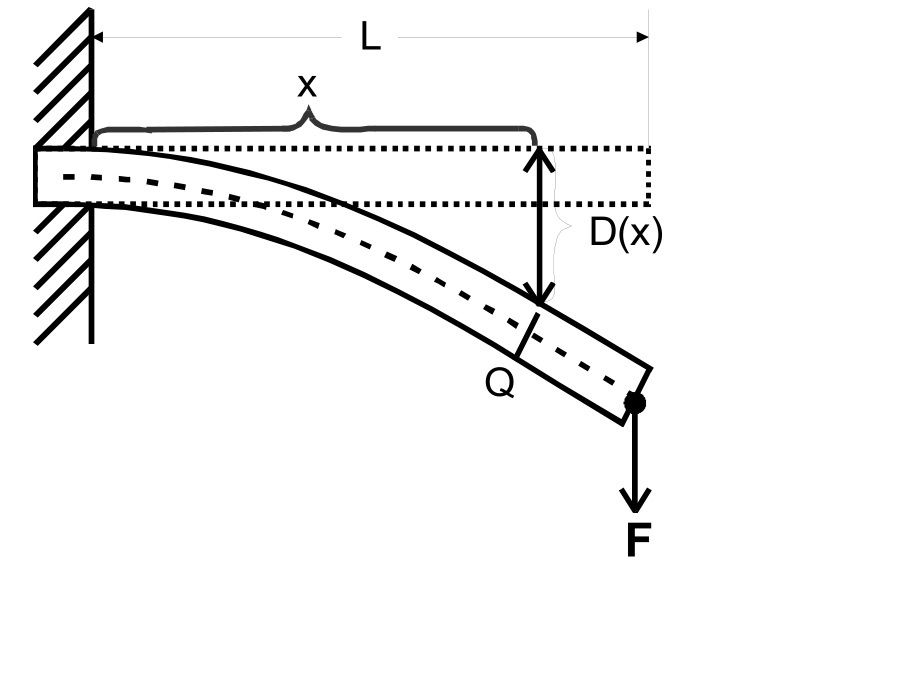
\includegraphics[0.5\textwidth]{content/data/biegen_einseitig.jpg}
    \caption{Stange mit Querschnitt $Q$ wird durch eine äußere Kraft $F$ einseitig gebogen.\cite{anleitung}}
    \label{fig:stab_einseitig}
\end{figure}
Die Kraft $F$ wirkt senkrecht auf den Querschnitt $Q$ des Stabes.
Sie bewirkt ein bestimmtes Drehmoment $M$ in Abstand $x$, das den Stab verbiegt.
Dabei werden obere Schichten gedehnt und die unteren gestaucht.
Durch die Elastizität des Materials stellt sich ein Gleichgewichtszustand und eine Durchbiegung $D$ ein.
In den oberen Schichten treten Zugspannungen auf, in den oberen Schichten Druckspannungen und dazwischen befindet sich ein Gebiet ohne Spannung.
Dieses Gebiet wird als neutrale Faser bezeichnet.
Das Drehmoment $M_\sigma$ berechnet sich nach
\begin{equation}
    M_\sigma = \int_Q y \sigma(y) \symup{d}q
\end{equation}